\section{Method}
\todo[inline]{New method introduction depending on how the disposition will be in the final form}
In order to answer the research questions stated in section~\ref{sec:RQ} a state of the art SPC, experiments and evaluation methods needs to be set up. In this section the SPC hardware and image sensing and reconstruction scheme is described.


\subsection{Single pixel camera architecture \& hardware}
\label{sec:system}
FOI designed the SWIR SPC platform using a DMD, a Newtonian telescope and a single pixel SWIR detector. The system also has a reference camera in the visual spectrum  which can capture images if all micro mirrors in the DMD are turned away from the single pixel sensor and towards the reference camera, it can also be used to check that the patterns are displayed correct on the DMD.  

\begin{figure}[H]
    \centering
    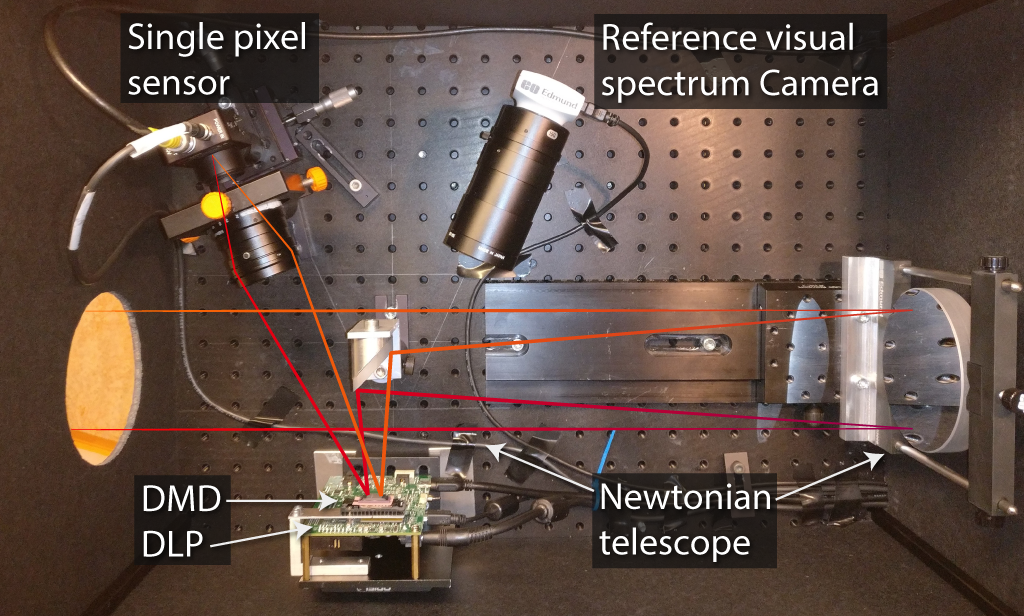
\includegraphics[width = 0.9\textwidth]{gfx/SPC.png}
    \caption{Single pixel imaging system (SPIS), adopted from \cite{article:foiSPIS}.}
    \label{fig:system1}
\end{figure}



As seen in figure~\ref{fig:system1} light from the scene is focused by the Newtonian telescope and reflected onto the DMD. The mirrors on the DMD can turned individually either into the single pixel sensor or the reference camera. The DMD acts as a Spatial Light Modulator (SLM) and reflects different patterns which is 'summed up' in the single pixel sensor as an intensity. The reconstructed image from the system will have the same resolution as the DMD patterns. The DLP is the DMD control unit which controls which patterns are displayed on the DMD either by reading images from memory or the video port.   


\subsubsection{Newtonian telescope}
A Newtonian telescope is a reflecting telescope, using a concave primary mirror and a flat diagonal secondary mirror, see figure~\ref{fig:system1}. In this set-up the telescope act as a lens focusing the scene onto the DMD. The motivation to use a Newtonian telescope instead of a lens system is partly that chromatic aberration is eliminated and partly that a reflective optical system works over a greater range of wavelengths that includes SWIR, near infrared (NIR) and the visible spectrum.

\subsubsection{DLP and DMD}
The DMD (Texas Instruments DLP4500NIR) is a matrix of micro mirrors that can be individually tilted $\pm 12^{\circ}$ and reflects wavelengths in the range 700-2500 nm. The DMD is controlled by the DLP (DLP LightCrafter 4500) which can be controlled either by video port (HDMI) or by the internal flash memory. The internal memory can theoretically be faster than the video port but due to constraints in both memory and memory bandwidth the fastest measurement matrix rate gets stuck at $270 - 300$ Hz. The video port can be operated at 120 Hz and display one bit plane at the time from a $24$ bit signal, which gives a maximum measurement matrix rate at $120 \times 24 = 2880$ Hz, but in the current configuration only $60$ Hz frame rate was achieved giving a measurement matrix rate at $1440$ Hz. At this rate with the number of measurements relative to number of pixels in reconstructed image between $20\% - 30\%$ a $256\times256$ pixel images data would be acquired in $9 - 13$ seconds and for a $512\times512$ pixel image $36-53$ seconds. To control the DMD the software 'DLP LightCrafter 4500 Control Software' is used.\\[0.1in] 

The DMD in the setup is constructed with a diamond shaped pattern instead of a regular square grid which is used in regular camera image sensors. The diamond shape causes the index of each mirror to be skewed against what a normal grid would look like. As seen in figure~\ref{fig:dmd_index} the indexes of the mirrors column is two mirror column arrays wide while a row is a single row. 


\begin{figure}[H]
    \centering
    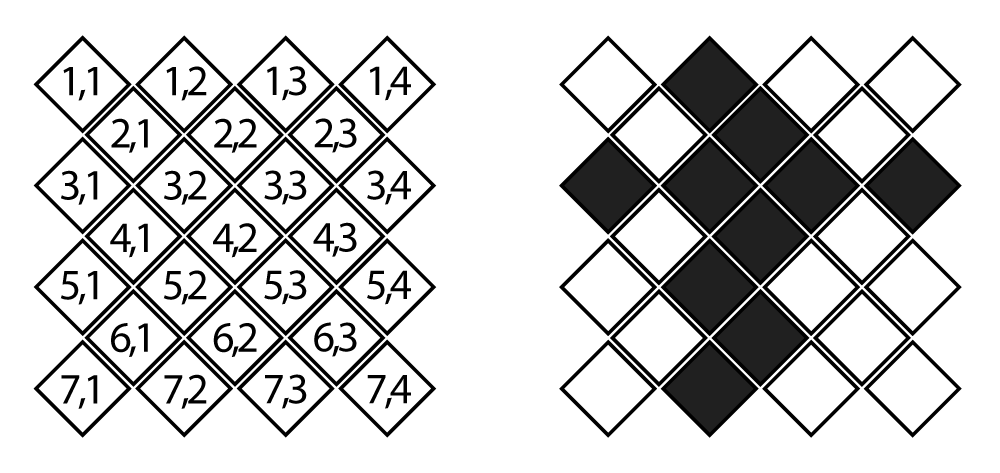
\includegraphics[width = 0.8\textwidth]{gfx/DMD_grid.png}
    \caption{DMD matrix, left shows each tiles index and right shows second row and second column in black.}
    \label{fig:dmd_index}
\end{figure}

Because the reconstruction algorithm and measurement matrix needs to be a square matrix with the side length with a power of 2 the resulting images ratio would be 2 to 1 while the image should have the ratio 1 to 1. The resulting image would need to be transformed into the real ratio where information potentially gets lost. Therefore the index of mirrors was changed so that each 'pixel' gets two mirrors as seen in figure~\ref{fig:dmd_index2}. This will result in rows and columns gets equal amount of space and the aspect ratio will be preserved to 1 to 1. 

\begin{figure}[H]
    \centering
    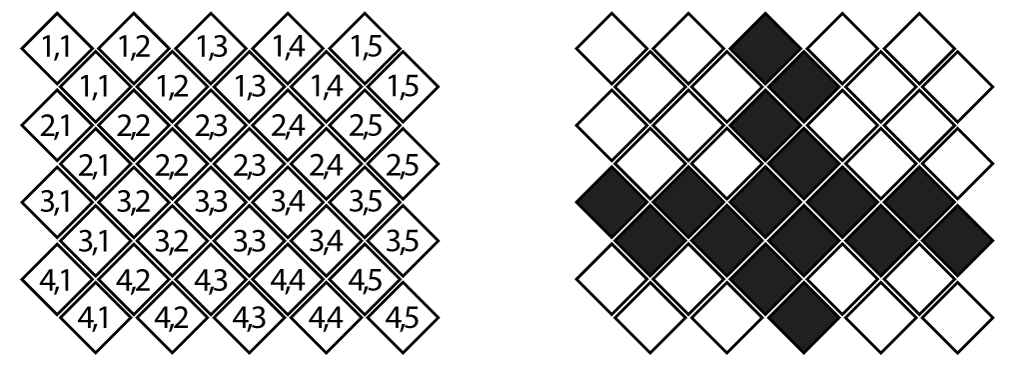
\includegraphics[width = 0.8\textwidth]{gfx/DMD_grid2.png}
    \caption{DMD matrix, left shows each tiles index and right shows third row and third column in black.}
    \label{fig:dmd_index2}
\end{figure}

\todo[inline]{Connect the DMD to CS and the physical aspect (every mirror is an pixel). I:I:D gaussian with DMD only can take values 1,0 gives 50\% evenly distrubitated pixels measurements for every measurement matrix which looks something like figure~\ref{fig:dmd_pattern}.} 


\begin{figure}[H]
    \centering
    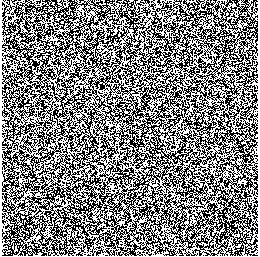
\includegraphics[width = 0.5\textwidth]{gfx/DMD_pattern.png}
    \caption{A typical measurement matrix presented on the DMD with the resolution $256 \times 256$ pixels.}
    \label{fig:dmd_pattern}
\end{figure}



\subsubsection{Lens}
The lens mounted on the single pixel sensor is an 50mm SWIR Fixed Focal Length Lens with an variable appature from f1.4 designed for wavelengths ranging from the 800 nm in the visual spectrum to 2000 nm in the SWIR spectrum. \cite{website:SWIR_objective}

\subsubsection{Single pixel sensor}
The single pixel sensor is a Thorlabs PDA20C/M and is sensitive in wavelength range 800-1700 nm which is beyond the visual spectrum (390-700 nm). The sensor outputs an analog signal in volt which the sampler converts to a discret value. \cite{manual:PDA}

\subsubsection{Signal spectrum}
All components characteristics assembled the wavelengths that pass trough the system and measured in the single pixel sensor is between 800-1700 nm.



\subsection{Compressive imaging}
\todo[inline]{Write introduction to CS, create some intuition}
The single pixel sensor captures a scene by measuring the light intensity focused into the detector reflected from the DMD matrix. The DMD sensing matrix changes to obtain new measurements, $M$ unique sensing matrix measurements is captured to reconstruct an image with $N$ pixels. Each sensing matrix index is encoded either  by a one or a zero (turning the mirror onto or away from the sensor). The compressive imaging sampling model is defined as

\begin{equation}
\label{eq:CS1}
   \mathbf{ y = \Phi x + \epsilon}\text{,}
\end{equation}\\[0.1in]


, $\mathbf{x}_{N\times1}$ is the signal (image) with $N$ samples (pixels), $\mathbf{y}_{M\times1}$ is the vector with $M$ measurements, $\mathbf{\Phi}_{M \times N}$ is the measurements matrix (each unique sensing matrix $\Phi_{1 \times N}$ as a row vector) and $\mathbf{\epsilon}$ is the noise. In conventional sampling the number of measurements $M$ needs to be at least equal to the number of samples $N$ to recover the signal but CS states that $M$ can be relatively small compared to $N$ given how compressible the signal is. The signal $\mathbf{x}$ can be represented as  

\begin{equation}
\label{eq:CS2}
   \mathbf{ \Psi \theta = x }\text{,}
\end{equation}\\[0.1in]

where, $\mathbf{\Psi}_{N \times N}$ is some  basis matrix and
$\mathbf{\theta}_{N\times1}$ is the coefficients where $\mathbf{\theta}$ is $K$-sparse. $K$-sparse means that the signal $\mathbf{x}$ has $K$ non zero elements in basis $\mathbf{\Psi}$, $||\mathbf{\theta}||_0 = K$. Given equation~\ref{eq:CS2}, equation~\ref{eq:CS1} can be expand to


\begin{equation}
   \mathbf{ y = \Phi x + \epsilon = \Phi \Psi \theta + \epsilon = A \theta + \epsilon }\text{,}
\end{equation}\\[0.1in]

where, $\textbf{A}_{M \times N} = \Phi \Psi$ is the reconstruction matrix. The last statement is what makes CS powerful, a signal which is not sparse can be sampled with measurement matrix $\Phi$ and then reconstructed with reconstruction matrix $\textbf{A}$ in a basis where $\textbf{x}$ is sparse or compressible. \cite{book:sm}

\todo[inline]{Noise dose not effect the measurement very much because half the intensity from the image is measured in one pixel sensor bumping the signal to noise ratio from a conv camera where each pixel has some noise half the pixels share that noise making SPC bery robust to noise even in low light situations. }

\subsection{Measurement matrix \& Restricted isometry property (RIP)}
\todo[inline]{Introduce the topic.}

In the noiseless case exact recovery of the image $\mathbf{x}$ is achievable if RIP holds for the reconstruction matrix $\mathbf{\Phi} \Rightarrow \mathbf{\Phi\Psi = A}$, the constraint is defined as,

\begin{equation}
    (1-\delta_K)||\mathbf{x}||_{\ell_2}^2\leq||\mathbf{Ax}||_{\ell_2}^2\leq(1+\delta_K)||\mathbf{x}||_{\ell_2}^2 \text{,}
\end{equation}\\[0.1in]

where $\delta_K \in [0.1)$ is the smallest constant to to satisfy RIP for a K-sparse signal $\mathbf{x}$. To determine a sampling matrix is a NP-hard problem (which means that there are no feasible way of creating a optimal reconstruction matrix) and generally $\textbf{x}$ is not known and varies which means that there are no general optimal reconstruction matrices for natural images. The solution is to find a general reconstruction matrix that satisfies RIP with high probability. The solution which also should be incoherent with the base matrix $\Psi$ is to construct the measurement matrix using a i.i.d random distribution which gives $\delta_K << 1$ with high probability. Using random measurement matrices the number of measurements needed to satisfy RIP with high probability is $M \geq O(K\text{log}(N/K) \ll N$. \cite{book:srr,article:CS_donoho1}\\[0.1in]

The problem using random matrices is that they need to be stored i memory for the reconstruction algorithm, when the image resolution is increased the measurement matrix increases exponentially. For images with resolution of $512\times 512$ and larger the data gets infeasible for a normal computer to handle.  Fortunately using fast transforms in the reconstruction algorithm can exclude using vector multiplication resulting in faster reconstruction and the need to store the measurement matrix in memory. But in order to do so special measurement matrices are used, in this master's thesis the sequency ordered Walsh Hadamard measurement matrix will be used with the TVAL3 reconstruction algorithm described in section~\ref{sec:TV}.   


\subsubsection{Sequency ordered Walsh Hadamard measurement matrix}
\label{sec:SOWHMM}
Besides from eliminating the need to store the measuring matrix for reconstruction the sequency ordered Walsh Hadamard (SOWH) matrix can be generated when sent to the DMD eliminating the need to store the matrix at all. SOWH has the same characteristics and properties of an i.i.d random matrix and therefore also fulfills the RIP condition with high probability and research has shown that there is no significant loss in recovery of the signal relative i.i.d random measurement matrix~\cite{article:an_improved_WH_matrix}.  An other property of SOHW is that it only contains -1 an 1 which easily be converted to 0 and 1 when sent to the DMD. \\[0.1in]


The naturally ordered Hadamard matrix of dimension $2^k$, $k \in \mathbb{N}$ are constructed by the recursive formula    

\begin{equation}
    H_0 = 1,
\end{equation}

\begin{equation}
    H_1 = \begin{bmatrix}
       1 & 1 \\
       1 & -1\\
     \end{bmatrix},
\end{equation}

and in general,

\begin{equation}
        H_k = \begin{bmatrix}
       H_{k-1} & H_{k-1} \\
       H_{k-1} & -H_{k-1}\\
       \end{bmatrix} = H_1 \oplus H_{k-1}
\end{equation}

where $\oplus$ denotes the Kronecker product. To construct the sequency ordered Walsh Hadamard matrix from the naturally ordered Hadamard matrix three steps is required:

\begin{itemize}
    \item Convert row index to binary.
    \item Convert the binary row index to gray code.
    \item Apply bit reverse on the gray code index.
\end{itemize}

then order the rows after the bit reverse to obtain the sequency ordered Walsh Hadamard matrix.

\begin{table}[H]
\begin{tabular}{|r|c|c|c|c|}
\hline
    $n_H$        & 0    & 1     & 2     & 3     \\ \hline
    Binary       & 00   & 01    & 10    & 11    \\ \hline
    Gray code    & 00   & 01    & 11    & 10    \\ \hline
    Bit-reverse  & 00   & 10    & 11    & 01    \\ \hline
    $n_W$        & 0    & 2     & 3     & 1     \\ \hline
    
\end{tabular}
\label{tab:Hadamard_2_Walsh}
\caption{How to convert a naturally ordered Hadamard matrix to a sequency ordered Walsh Hadamard matrix by shifting row with index $n_W$ to $n_H$}
\end{table}

for example

\begin{equation}
    H_2 =  \begin{bmatrix}
       1 & 1 & 1 & 1 \\
       1 & -1 & 1 & -1 \\
       1 & 1 & -1 & -1 \\
       1 & -1 & -1 & 1 
       \end{bmatrix} \Rightarrow W_2 = \begin{bmatrix}
       1 & 1 & 1 & 1 \\
       1 & 1 & -1 & -1  \\
       1 & -1 & -1 & 1  \\
       1 & -1 & 1 & -1 
       \end{bmatrix}.
\end{equation}

To use the sequency ordered Walsh Hadamard matrix as an measurement matrix the fist row is omitted, permutations to the columns is performed, $M$ rows are choosen at random and the indices with a $-1$ is shifted to $0$. This last step is required to convert the measurement matrix so it gets the characteristics of an i.i.d random matrix and thus fulfill the RIP condition~\cite{article:SRM_long, article:WH_RIP_SRM, article:WH_mixed_RIP_prof}. How the matrix was permutated and which rows was choosen i which order is stored so the reconstruction algorithm can use that information. \cite{article:SRM_long, article:TVAL3, article:an_improved_WH_matrix}. 

\todo[inline]{permutation is not nessesary?}

\subsection{Reconstruction method}
To reconstruct the image $\textbf{x}$ the sparest set of coefficients in $\theta$ is desired. The optimal approach to find these coefficients would be to use $\ell_0$ minimization


\begin{equation}
   \mathbf{ \hat{\theta}} = \text{arg min } ||\mathbf{\theta}||_0 \text{  subject to  } \mathbf{y = A\theta} \text{.}
\end{equation}\\[0.1in]


Simply minimizing nonzero indices $\mathbf{\theta}$ in the sparsitfying basis $\mathbf{\Psi}$, but this problem is known to be NP-hard. A better approach is the $\ell_1$ minimization, for example Basis Pursuit denoise (BPDN),

\begin{equation}
    \mathbf{\hat{\theta}} = \text{arg min } ||\mathbf{\theta}||_1 \text{  subject to  } ||\mathbf{y - A\theta}||_2 < \mathbf{\epsilon} \text{.}
\end{equation}\\[0.1in]


In 2006 Donoho~\cite{article:CS_donoho1} for the fist time guarantied theoretical $\ell_0\text{/}\ell_1$ equivalence which holds in the CS case, which means using a $\ell_1$ minimizer is guaranteed to find the sparsest solution in polynomial time in the noiseless case which can be approximated in the noisy and compressible signal case. The drawback with the $\ell_1$ minimizer is that it require more measurements than the optimal case with $\ell_0$ but it is still $M \ll N$. Since 2006 many more types of optimization algorithms has evolved which solves the problem with different methods but with the same goal: finding the largest most significant coefficients of $\mathbf{\theta}$. \cite{article:CS_donoho1, article:single_pixel_im_cs, article:a_new_ci_arc}


\subsubsection{Total variation: TVAL3}
\label{sec:TV}
The reconstruction algorithm that was chosen in this Master's thesis was a total variation regularization algorithm. Natural images often contains sharp edges and piecewise smooth areas which the TV regularization algorithm is good at preserving. The main difference between TV an other reconstruction algorithms is that TV considers the gradient of signal sparse instead of the signal, thus finding the sparsest gradient. The TV optimization problem in TVAL3 is defined as  

\begin{equation}
\text{min}_\mathbf{x} \Sigma_i ||D_i \mathbf{x} || \text{, subject to } \mathbf{\Phi x} = 	y \text{, } \mathbf{x} \geq 0 \text{,} 
\end{equation}

where $D_i\mathbf{x}$ is the discrete gradient of $\mathbf{x}$ at position $i$.\\[0.1in]

TVAL3 stands for "Total Variation Augmented Lagrangian Alternating Direction Algorithm", accordingly is a TV regularization algorithm which uses augmented Lagrangian and alternating direction methods, where augmented Lagrangian is a method in optimization for solving constrained problems by substitute the original constrained problem with a series unconstrained subproblems and introduce a penalty term. To solve the new subproblems the alterning direction method is used~\cite{article:TVAL3}.\\[0.1in]

As mentioned earlier in section~\ref{sec:SOWHMM} the main reason why the sequency ordered Walsh Hadamard matrix is used is to eliminate the need to store the matrix in memory during reconstruction and a promise to speed up the reconstruction. In TVAL3 there are two multiplications between matrix and a vector that dominates the computation time,

\begin{equation}
\mathbf{\Phi}\mathbf{x}^k \text{ and } \mathbf{\Phi}^\top(\mathbf{\Phi}\mathbf{x}^k-\mathbf{y})\text{.}
\end{equation}

The idea is to replace the multiplication with fast transforms. To explain the concept some observations and new functions need to be defined. The first observation is that the sequency ordered Walsh Hadamard matrix is a transform matrix which also can be computed with the fast Walsh Hadamard transform (fwht),

\begin{equation}
\mathbf{W}\mathbf{x} = \text{ fwht}(\mathbf{x}),
\end{equation}

where $W$ is a sequency ordered Walsh Hadamard matrix and $\mathbf{x}$ is the signal vector. The wht is a generalized class of Fourier transforms which decomposes input vector into superposition of Walsh functions.\\[0.1in]

From section~\ref{sec:SOWHMM} it was briefly mention in the last paragraph that in order for the measurement matrix to fulfill RIP the columns is permutated and rows are chosen in random to create the measurement matrix from the sequency ordered Walsh Hadamard matrix, two functions is created to carry out does operations. First the permutation function $\pi(\cdot)$, which from a random seed permutate the order of the columns in a matrix or the order of a vector. The second function $\Pi_M(\cdot)$ chooses $M$ row in a matrix at random and stacks them in a new matrix. Then the definition of the measurement matrix $\mathbf{\Phi}$ constructed from the sequency ordered Walsh Hadamard matrix $\mathbf{W}$ leads to observation 2

\begin{equation}
\mathbf{\Phi} = \pi(\Pi_M(\mathbf{W})) = \Pi_M(\pi(\mathbf{W}))\text{.}
\end{equation}

It does not matter in which order the functions i applied, it gives the same result. With matrix $\mathbf{A}$ and vector $\mathbf{u}$ observation 3 is formulated as,

\begin{equation}
\pi(\mathbf{A})\mathbf{u} = \mathbf{A}\pi(\mathbf{u})\text{,}
\end{equation}

which shows that there is no difference between multiply a column-permutated matrix with a vector and multiply the same matrix with the vector permutated.\\[0.1in]

With all observations combined the matrix multiplication is replaced with the fwht in observation 4

\begin{equation}
\mathbf{y} = \mathbf{\Phi}\mathbf{x} = \pi(\Pi_M(\mathbf{W}))\mathbf{x} = \Pi_M(\mathbf{W})\pi(\mathbf{x}) = \Pi_M(\mathbf{W}\pi(\mathbf{x})) = \Pi_M(\text{fwht}(\pi(\mathbf{x}))\text{,}
\end{equation}

with the conclusion that the multiplication between the measurement matrix constructed using the permutated sequency ordered Walsh Hadamard matrix and the signal can be performed with the signal permutated, fast transformed using fwht and choosing rows, both permutations using the same functions $\pi(\cdot) \text{ and } \Pi_M(\cdot)$ and random seed as when the measurement matrix was created.\\[0.1in]

Using this method will reduce the overall computational complexity considerably and it will make the measurement matrix redundant in the reconstruction, only the two permutation functions $\pi(\cdot) \text{ and } \Pi_M(\cdot)$ needs to be stored. Excluding the measurement matrix in the reconstruction results in larger resolution images ($512\times512$ pixels and larger) can be reconstructed. \cite{article:SRM_long, article:TVAL3}



\subsection{Image capturing and processing chain}
To capture an image the SPC setup is only a subsystem in the whole process from acquiring the signal to reconstructing the image. In figure~\ref{fig:flow_chart} the whole process of capturing an image is presented with all subsystems and signal/image processing steps included.

\begin{figure}[H]
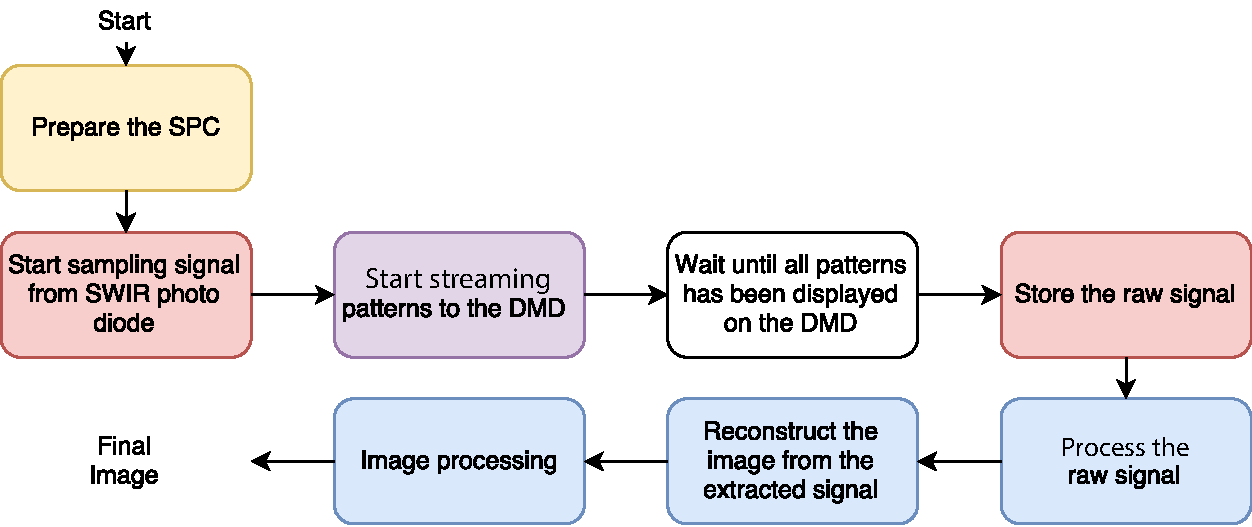
\includegraphics[width = 1\linewidth]{gfx/flowchart3.pdf}
\caption{Block diagram of image capturing and processing chain, from signal acquisition to final image. Each color represents different subsystems in hardware or software.}
	\label{fig:flow_chart}
\end{figure}

This experimental setup has no full automatic system where a button can be pressed and the system produces an image. In the setup the subsystems works completely independently and needs to be operated manually in the right order at the right time. Each color in figure~\ref{fig:flow_chart} represents a subsystem in hardware or software. Each subsystem is be described in the following subsection.

 
\subsubsection{Prepare the SPC}
The first step in the yellow block "Prepare the SPC" is making sure the SPC is up and running but also to point the camera at the scene and set the correct focus. The scene is located with the aid of the reference visual camera (see figure~\ref{fig:system1}) with all the mirrors in the DMD directed to that camera. The focus is adjusted manually by moving the primary mirror back or forth, this procedure may introduce some error to the focus.\\[0.1in]

\subsubsection{Sampling}
The red blocks subsystem "Start sampling signal from SWIR photo diode" and "Store the raw signal" is conducted in a separate software which controls the A/D converter and thus the sampling. When the SPC i prepared the sampling of the signal is started with sampling rate such that every measurement has several sampling points thus oversampling the signal. The oversampling is needed because when the mirrors move from one pattern (measurement matrix) to the next the signal is uncertain for some time, the oversampling is also used to suppress noise from the photo diode, more on that in section~\ref{sec:signal_process}. After the signal is sampled the obtained signal needs to be stored on the computer manually.

\subsubsection{Streaming patterns to the DMD}
\label{sec:stream_dmd}
The subsystem "Streaming patterns to the DMD" represented in purple in the block diagram is controlled by two different softwares, one which manipulates the pattern-signal received by the DMD and one which sends the patterns to the DMD. The patterns are sent to the DMD through a HDMI cable where the DMD is set up such that the DMD acts as an second screen to the computer. This enables to show anything on the DMD that a screen can show. The patterns are stored as a video and played back on the DMD "screen" with a media player which shows each pattern in consecutive order. This is the major bottleneck of the system where each measurement matrix needs to be displayed one after the other depending on how fast frame rate can be achieved. The naive approach would be to display one pattern per frame which is linked to the frame rate of the DMD, lets say for example 60 frames per second (fps) then for a $512\times 512$ pixel large image sampled with $M/N = 20\%$ measurement matrices gives $52428$ patterns which would take $52428/60 = 874 \text{ seconds} = 14.5 \text{ minutes}$ to sample which is a long exposure time for a still image with the constraint that the scene should be stationary to obtain a stationary signal.\\[0.1in]

Fortunately with the software "DLP LightCrafter 4500 EVM GUI" controlling the DMD the received video signal can be manipulated before displayed onto the DMD. The software includes a function which can break down the received 24-bit color image into 1 bit planes which can be displayed in consecutive order, so for each frame received 24 patterns is encoded on that frame then the DMD software isolates each bit plane and displays them in consecutive order. This function improves the naive implementation by a factor of $24$, which reduces the time to sample the image from the last example from $874 \text{ seconds to } 874/24 = 36 \text{ seconds}$. This exposure time is of course not optimal for natural images outdoors but acceptably for the experimental setup.\\[0.1in]     


To create the video that feeds the patterns to the DMD each pattern  i.e. measurement matrix is created as presented in section~\ref{sec:SOWHMM}. Then for each group of 8 unique patterns drawn from the rows of the measurement matrix are stacked in each bit plane of a 8 bit image as seen in figure~\ref{fig:8_to_1_8}.

\begin{figure}[H]
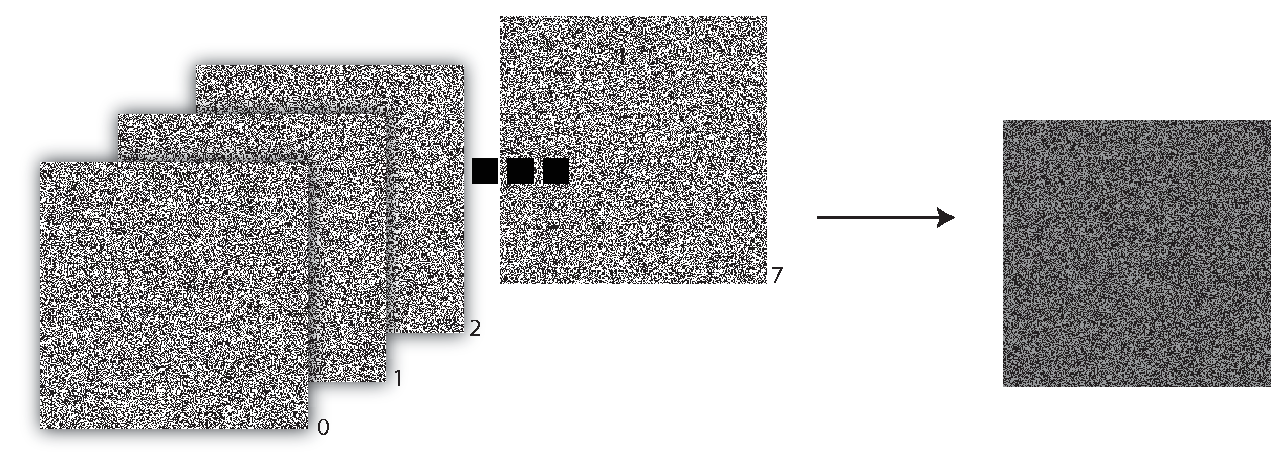
\includegraphics[width = 1\linewidth]{gfx/DMD_12.eps}
\caption{Stack each group of 8 measurement matrices in separate  bit planes creating one 8 bit image with each matrix in one bit plane.}
	\label{fig:8_to_1_8}
\end{figure}

Then for each group of three 8 bit images a 24 bit color image is constructed as seen in figure~\ref{fig:3_8_to_1_3}. 

\begin{figure}[H]
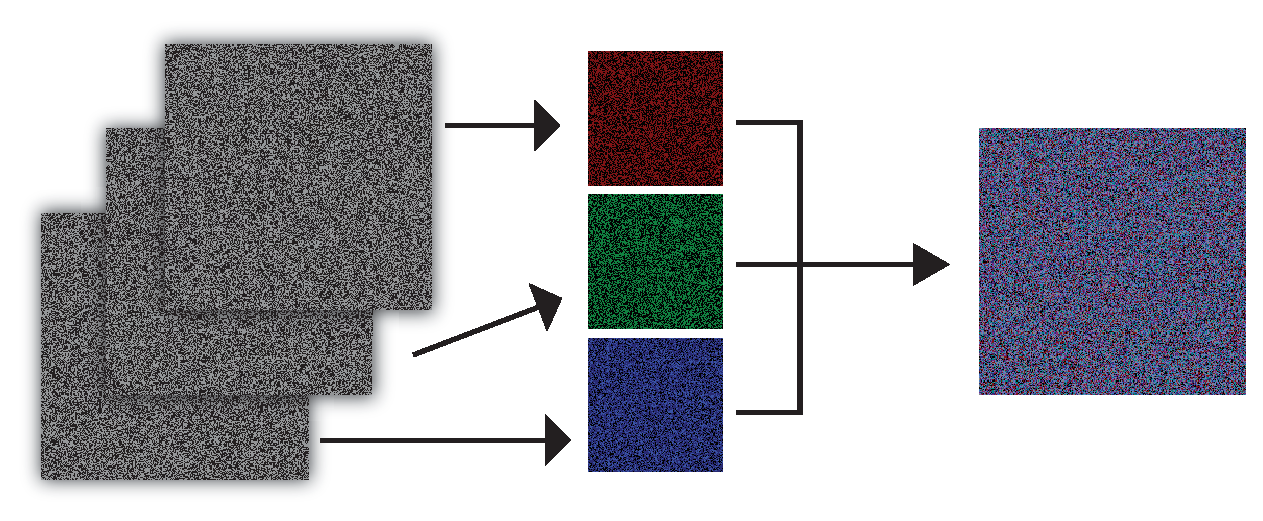
\includegraphics[width = 1\linewidth]{gfx/DMD_2.eps}
\caption{Stack each group of three 8 bit plane images into one 24 bit color image. This is one frame in the video sent to the DMD.}
	\label{fig:3_8_to_1_3}
\end{figure}

This 24 bit color image corresponds to one frame in the video, to create the video this is done so each pattern is represented in the video.



\subsubsection{Signal processing}
\label{sec:signal_process}  
When the sampled signal is stored on the computer the remaining signal/image processing and reconstruction represented by blue blocks in figure~\ref{fig:flow_chart} is conducted in MATLAB. In this section the signal processing of the sampled signal is described.\\[0.1in]

The first step is to refine the raw over sampled signal so that each measurement matrix correspond to one measurement in signal $\mathbf{y}$. This is done by first find every set of indices corresponds to every measurement matrix, as seen in figure~\ref{fig:raw_signal} where the signal indices which corresponds to one measurement matrix is isolated by the purple lines.


\begin{figure}[H]
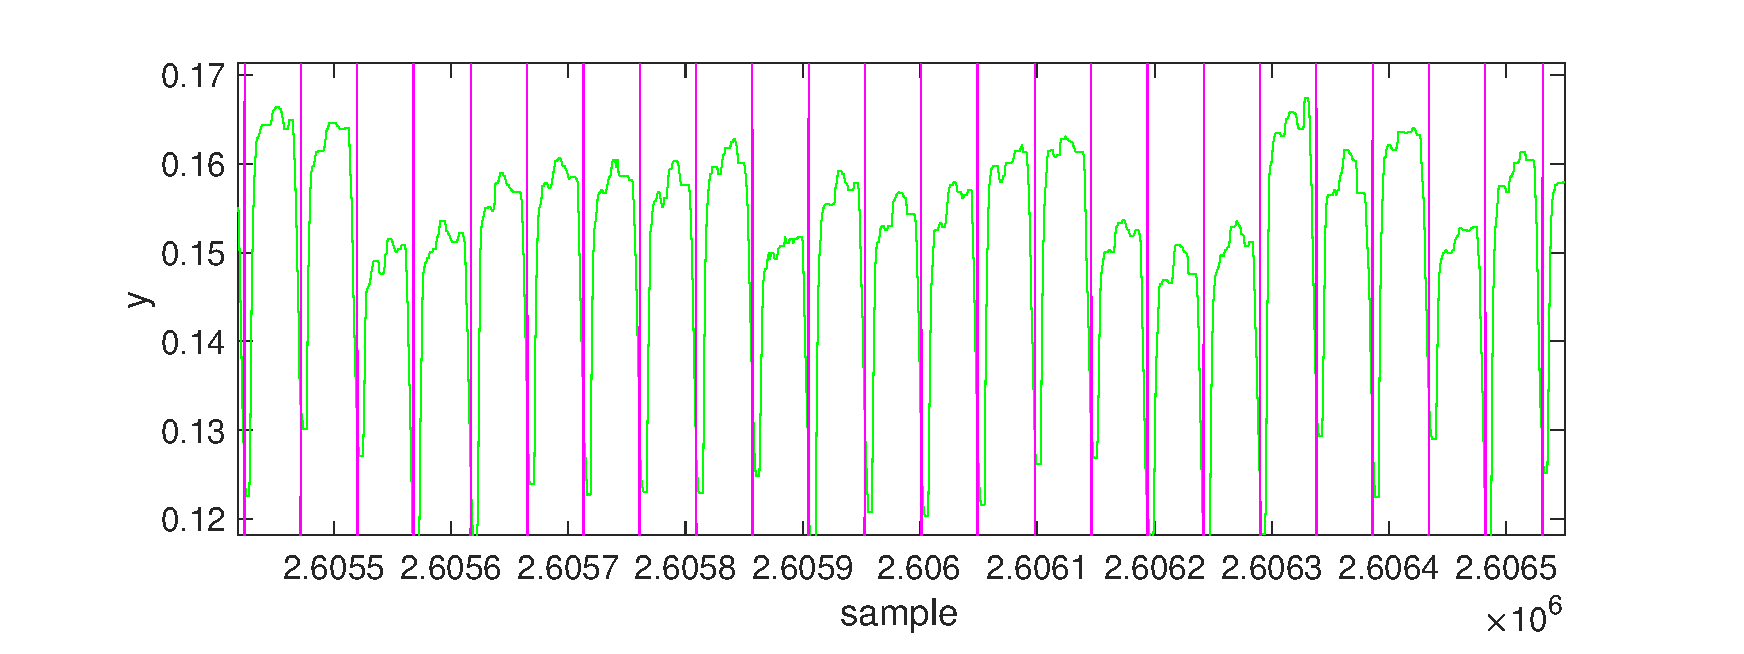
\includegraphics[width = 1\linewidth]{gfx/signal_proc/isolated_raw_signal.eps}
\caption{---}
	\label{fig:raw_signal}
\end{figure}

The next step is to determine one value for each measurement. This is done in two steps the first is to omit values which corresponds to the DMD changing pattern seen in figure~\ref{fig:raw_signal} where the purple line divides the measurements the DMD is changing pattern which gives an uncertain signal. With the omitted parts of the signal corresponding to one measurement the mean is calculated and set to the value for each measurement, as seen in figure~\ref{fig:detarmain_signal}. 

\begin{figure}[H]
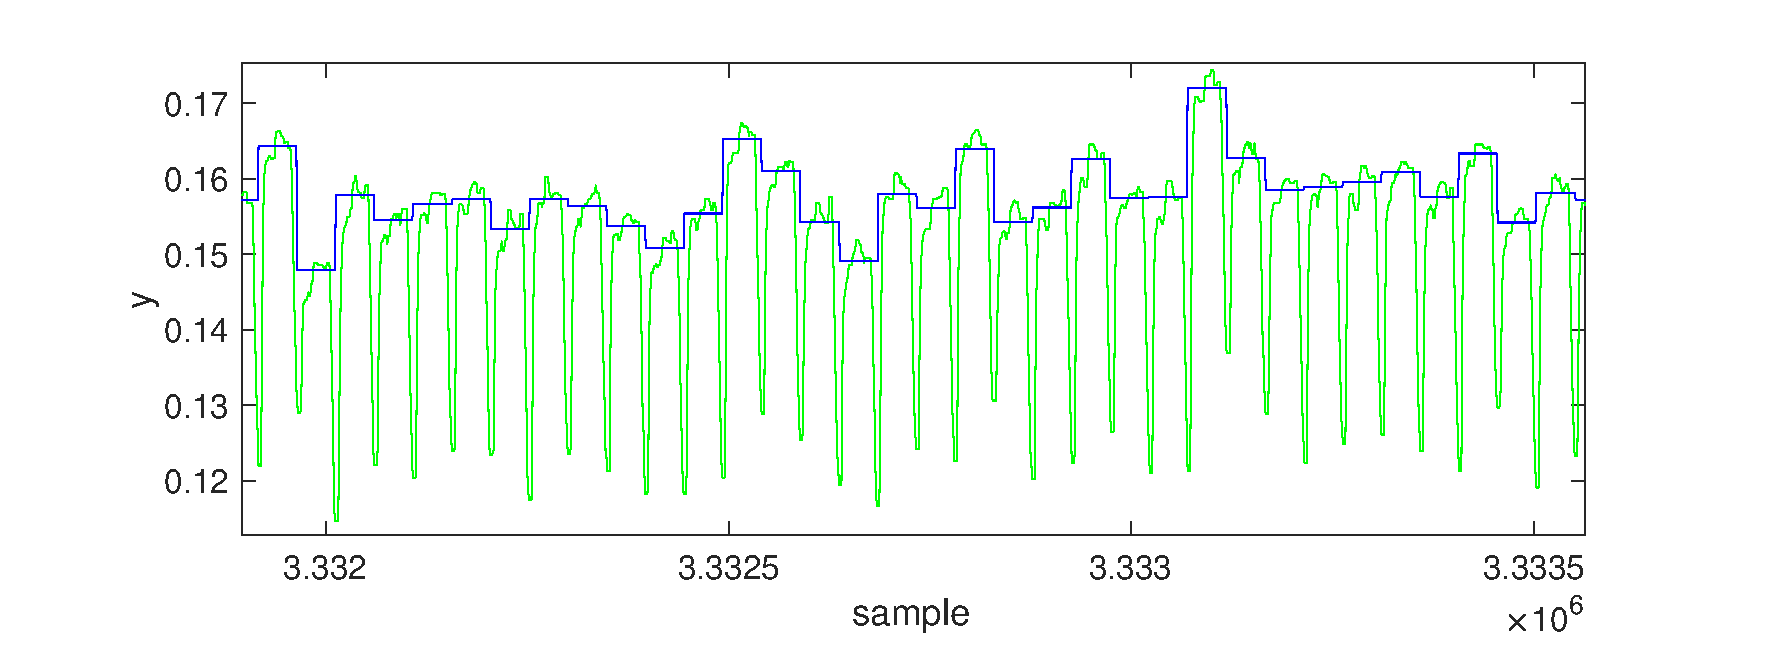
\includegraphics[width = 1\linewidth]{gfx/signal_proc/isolated_final_signal.eps}
\caption{---}
	\label{fig:detarmain_signal}
\end{figure}



\subsubsection{Dynamics in scene} %: luminance change}
\label{sec:Dynamics_in_scene}
So far the measurement vector $\mathbf{y}$ has been determined, in the ideal case even with added noise the measured signal should be stationary because the image is assumed to be constant with half the pixels measured at random uniformed spread across the image. Each pixel in the image has the same value in each measurement with some noise added which is divided by all pixels being measured	 i.e. half the pixels which does not have a significant impact of the reconstructed image. But when capturing images outdoors with natural light in addition with long exposure time as described in section~\ref{sec:stream_dmd} it is not certain that the image (or every pixel) is constant over the exposure time which will reduce reconstruction performance because of the ambiguity of each pixel. The potential dynamics in a scene can be divided into two categories: luminance change and object movement. In this subsection the luminance change problem is modeled with corresponding algorithm to suppress the impact on the reconstructed image. The object movement problem will not be modeled, instead be avoided when capturing the signal by making sure the scene is as static as possible.\\[0.1in] 


In natural outdoor images it can be assumed the the primary source of light comes from the sun, but even on a clear day the light intensity from the sun is not constant. If the scene is assumed to be completely stationary even the slightest intensity change will be added for all pixels being measured changing the mean intensity of the measured signal $\mathbf{y}$ which should be stationary. With the assumption that the image is constant and the luminance change uniformly adds the same intensity to each pixel per measurement the problem can be modeled.\\[0.1in]

Start of with the original theorem and disregard the noise, 

\begin{equation}
\mathbf{y} = \mathbf{\Phi}\mathbf{x},
\end{equation}  

the image $\mathbf{x}$ can not longer be considered constant for all measurements, the luminance change will change image $\mathbf{x}$ for every measurement matrix $\mathbf{\Phi}_i$ depending on the uniform luminance change. This can be described for one measurement as,  

\begin{equation}
y_i = \mathbf{\Phi}_i\mathbf{x}_i = \mathbf{\Phi}_i(\mathbf{x} + \mathbf{l}_i) = \mathbf{\Phi}_i\mathbf{x} + \mathbf{\Phi}_i\mathbf{l}_i ,
\end{equation}
  
where $\mathbf{l}_i$ uniform adds the same intensity over the whole image $\mathbf{x}$ for measurement $i$. It is known from before that the measurement matrix $\mathbf{\Phi}_i$ contains $50\%$ zeros and ones which gives,

\begin{equation}
y_i = \mathbf{\Phi}_i\mathbf{x} + \mathbf{\Phi}_i\mathbf{l}_i = \mathbf{\Phi}_i\mathbf{x} + \frac{N}{2}c_i,
\end{equation}

where $c_i$ is the uniform intensity change coefficient for measurement $i$. This function can be generalized for all measurements,

\begin{equation}
\mathbf{y} = \mathbf{\Phi}\mathbf{x} + \frac{N}{2}c_i = \mathbf{\Phi}\mathbf{x} + \mathbf{c},
\end{equation}

where $\mathbf{c}$ is the intensity change vector.\\[0.1in]

The goal is now to remove the intensity change vector from signal $\mathbf{y}$. Using the knowledge that the signal $\mathbf{y}$ should be stationary and assumes that the rate of change in intensity has a much lower frequency than the intensity change between individual measurement matrices, then $\mathbf{c}$ can be approximated by the moving average and simply removed from signal $\mathbf{y}$. The moving average is calculated at each data point in the signal vector $\mathbf{y}$ by calculating the average of $k$ points centered around the data point.    
		 
		 
%\subsubsection{Dynamics in scene: structure movement}
%Moving objects in the scene is more complex problem than the previous luminance change, both detecting the movement by reading the measured signal and if detected how to remove the problem. In this master's thesis scenes which is known to contain large movement will be avoided, while some small movement for example created by the wind will have to be accepted. In this section a method i proposed to detect a large object rapidly moving in and out of the scene  
%
%In this section a model of a static      

\subsubsection{Reconstruction}
Reconstruction is performed using the TVAL3 algorithm described in section~\ref{sec:TV}. The algorithm takes in measurement matrix $\mathbf{\Phi}$, signal $\mathbf{y}$ and algorithm settings as arguments and outputs the reconstructed image. The setting used throughout all experments is:

\begin{itemize}
\item \textit{opts.mu} $= 2024$
\item \textit{opts.beta} $= 64$
\item \textit{opts.maxcnt} $= 10$
\item \textit{opts.maxit} $= 1000$
\item \textit{opts.tol\_inn} $= 10^{-5}$
\item \textit{opts.tol} $= 10^{-10}$ 
\item \textit{opts.mu0} $= 2^4$ 
\item \textit{opts.beta0} $= 2^0$
\item \textit{opts.nonneg} $=$ true 
\item \textit{opts.isreal} $=$ true	
\end{itemize} 

Which solves for a real non negative solution described in section~\ref{sec:TV}. 


\subsubsection{Image processing}
From the reconstructed image some light image processing is done. There are only two operations applied to the reconstructed image and the reason why is that the images presented in the evaluation should represent what can be expected from the system. Furthermore often image processing is applied on special problems or artifacts in the images and it is not desired to cover up if there exist such problems. Therefore the two operations used is median filter and adjusting the intensity for higher contrast.\\[0.1in]

The reconstructed image has a high dynamic range and if only a small set of neighboring pixels is reconstructed with a high intensity peak which not correlates to the rest of the image these pixels will drop the contrast in the rest of the image, to remove these peaks the median filter is used. The median filter will also remove "salt and pepper" noise while edges are preserved. The built in MATLAB function \textit{medfilt2} will be used.\\[0.1in]

The second operation is an intensity transform to maximize the contrast in the image, the built in MATLAB function \textit{imadjust} will be used.   


\subsection{Evaluation: Image quality assessment}
\label{sec:method_eval}
The evaluation will be divided in to two categories: reconstructed images from synthetic data and images reconstructed from data acquired by the SPC.\\[0.1in] 

The evaluation on synthetic data is focused on evaluating the performance of the measurement matrix and reconstruction algorithm. Evaluating synthetic data gives two possibilities that can not be achieved with images reconstructed using the SPC which is that there is a reference image which the resulting image can be compared to.

Reconstructed image from synthetic data is acquired by creating a signal $ \mathbf{ y }_{M\times1}$ taking the inner product of $ \mathbf{y} = \mathbf{\Phi} \mathbf{x} + \epsilon$ where, $\mathbf{x}$ is the synthetic image reshaped to a vector, $\mathbf{\Phi}$ is the measurement matrix with the desired amount of measurements $M$ and synthetic noise $\epsilon$ which can be regulated to simulate different conditions, then using the reconstruction algorithm on the signal $\mathbf{y}$ to obtain the reconstructed image $\mathbf{\hat x}$. Because the measurement matrix and reconstruction algorithm is independent of the SPC hardware the subsystem can be evaluated independently. Two advantages of evaluation the sensing and reconstruction independently of the SPC is that parameters such as number of measurements and noise can be regulated easy and the second advantage is that a reference image is available for comparison.\\[0.1in] 

With a reference image available two image quality assessments are performed on the result from the simulation: Peak signal-to-noise ratio (PSNR) and  SSIM. PSNR is defined as

\begin{equation}
    \text{PSNR}[f(x,y),g(x,y)] = 10 log_{10}\frac{E^2}{\text{MSE}[f(x,y),g(x,y)]}
\end{equation}
 
where, $f(x,y)$ and $g(x,y)$ is intensity in pixel $(x,y)$ and MSE is the mean square error between the images defined as

\begin{equation}
\text{MSE}[f(x,y),g(x,y)] = \frac{1}{mn}\sum_{x=0}^{y-1}\sum_{n=0}^{n-1}[f(x,y) - g(x,y)]^2.
\end{equation}
 
 

\pagebreak
\todo[inline]{Large syntetic test of SWIR images, Whar result can be expected}

\todo[inline]{Synthetic test of the methods presented in section~\ref{sec:signal_process} will be conducted to measure the performance and validity.}

\todo[inline]{Number of measurements needed to get a good image}

\todo[inline]{Homography test}

\todo[inline]{Brisque}

\todo[inline]{MTF which measures Edge response}


\subsection{Method criticism}
\begin{itemize}
    \item No Reference Image Quality Assessment is not designed for SWIR images or SPC:s characteristics noise therefore the results may not reflect how the QA would answer to visual wavelength cameras. 
\end{itemize}
%LSE - absolute error but does not say much about how humans perceives the image.\\

